\documentclass[
  xcolor={svgnames},
  hyperref={unicode=true,colorlinks,citecolor=DeepPink4,linkcolor=DarkRed,urlcolor=DarkBlue}
  ]{beamer}
\usepackage[utf8]{inputenc}
\usepackage[bulgarian]{babel}
\usepackage{amsmath}
\usepackage{amssymb}
\usepackage{amsthm}
\usepackage{lmodern}
\usepackage{mathtools}
\usepackage{yfonts}
\usepackage{indentfirst}
\usepackage{comment}
\usepackage{eurosym}
\usepackage{textcomp}
\usepackage{subcaption}
\usepackage{graphicx}
\usepackage{tabto}
\usepackage{datetime}

\usetheme{Frankfurt}
%\usetheme{Copenhagen}
%\usetheme{Malmoe}
\usecolortheme[named=black]{structure}
\beamertemplatenavigationsymbolsempty

\DeclareFontShape{OT1}{cmss}{b}{n}{<->ssub * cmss/bx/n}{}

\begin{comment}
\useoutertheme{}
\setbeamertemplate{headline}
{%
  \leavevmode%
  \begin{beamercolorbox}[wd=.5\paperwidth,ht=2.5ex,dp=1.125ex]{section in head/foot}%
    \hbox to .5\paperwidth{\hfil\insertsectionhead\hfil}
  \end{beamercolorbox}%
  \begin{beamercolorbox}[wd=.5\paperwidth,ht=2.5ex,dp=1.125ex]{subsection in head/foot}%
    \hbox to .5\paperwidth{\hfil\insertsubsectionhead\hfil}
  \end{beamercolorbox}%
}

\setbeamertemplate{navigation symbols}{Frankfurt}


\pagecolor[rgb]{0.19,0.19,0.19}
\color[rgb]{0.77,0.77,0.77}
\setbeamercolor{palette primary}{bg=white,fg=black}
\setbeamercolor{palette secondary}{bg=white,fg=black}
\setbeamercolor{palette tertiary}{bg=white,fg=black}
\setbeamercolor{palette quaternary}{bg=white,fg=black}
\setbeamercolor{structure}{fg=black} % itemize, enumerate, etc
\setbeamercolor{section in toc}{fg=black} % TOC sections

\end{comment}




\title{Модел на сезонна миграция}
\subtitle{Проект по "Въведение в изчислителната биология"}
\author{изготвил: Калоян Стоилов \\ ръководител: Петър Рашков}
\date{\formatdate{8}{2}{2021}}

\begin{comment}
\institute{Софийски университет "Св. Климент Охридски" \\ Факултет по математика и информатика}
\end{comment}

\institute{\textbf{\textit{СОФИЙСКИ УНИВЕРСИТЕТ \\ "СВ. КЛИМЕНТ ОХРИДСКИ"}}
\begin{center}

\includegraphics[width=1.2cm,height=1.5cm]{logo_su_s_nadpis_imagelarge}
\end{center}
ФАКУЛТЕТ ПО МАТЕМАТИКА И ИНФОРМАТИКА
}


\begin{document}

{
\setbeamertemplate{headline}[default]

\begin{frame}
\titlepage
\end{frame}

}

%\section{Динамика на Бевъртън-Холт}

\begin{frame}[t]{Динамика на Бевъртън-Холт}

  Динамиката на Бевертън-Холт е вид популационна динамика, където $x(n+1)=\frac{\lambda x(n)}{1+bx(n)}$. Моделът който ще разглеждаме, ще се базира на тази динамика. Предполагаме наличието на две местности, които обитава някой вид. Също така времето е разделено на периоди така, че се редуват:
  \begin{itemize}
    \item период на размножаване във всяка от териториите
    \item период на размножаване с миграция на индивиди
  \end{itemize}

\end{frame}

\begin{frame}[t]{Формулировка на миграционния модел}

  Когато n е четно, то имаме следната динамика:
  \[x_{1}(n+1)=x_{1}(n)\frac{a_{1}}{1+b_{1} x_{1}(n)}\]
  \[x_{2}(n+1)=x_{2}(n)\frac{a_{2}}{1+b_{2} x_{2}(n)}\]

  Когато n е нечетно, то тя е:
  \[x_{1}(n+1)=(1-d_{1})x_{1}(n)\frac{\alpha_{1}}{1+\beta_{1} x_{1}(n)} + d_{2} x_{2}(n)\frac{\alpha_{2}}{1 + \beta_{2} x_{2}(n)}\]
  \[x_{2}(n+1)=d_{1}x_{1}(n)\frac{\alpha_{1}}{1+\beta_{1} x_{1}(n)} + (1-d_{2}) x_{2}(n)\frac{\alpha_{2}}{1 + \beta_{2} x_{2}(n)}\]

  Стойностите на параметрите удовлетворяват:
  $\alpha_{i},  \beta_{i}, a_{i}, b_{i} > 0,$ $i=1,2$ и приемаме, че $a_{i} \neq \alpha_{i}, b_{i} \neq \beta_{i}, i=1,2$.
  
\end{frame}


\begin{frame}[t]{Задача 1}
  Обяснете какви стойности трябва да приемат параметрите, за да бъдат гъстотите на популациите строго неотрицателни, т.е. да е изпълнено $x_{i}(n) \geq 0, n \geq 1$.
\end{frame}


%\section{Параметрите и стойностите им}

\begin{frame}[t]{Параметрите и стойностите им}

Параметрите трябва да са такива, че моделът да е дефиниран за всяко $n \geq 0$, както и при задаване на правдоподобни стойности - неотрицателни числа като начални условия, то да имаме и $x_{i}(n) \geq 0, n \geq 0, \; i=1,2$. Също така трябва да отчетем, че при някои стойности на параметри моделът може да се изроди в друг. 

\end{frame}


\begin{frame}[t]{Параметрите и стойностите им}

Желаем това от параметрите, тъй като при $b_{i}=0$ моделът се изражда в експоненциален, а при $a_{i}=0$ просто $x_{i}(n+1)=0$. Желаем неотрицателността им, тъй като при $b_{i} < 0$, имаме $x_{i} = 1/b_{i}$ води до недефинираност на модела, а при $a_{i} < 0 $, то $sgn(x_{i}(n+1)) = - sgn(x_{i}(n))$, поне при $x_{i} < 1/b_{i}$. Също така при $b_{i} < 0$, ако $x_{i} > 1/b_{i}$, при $a_{i} > 0 $, то отново $sgn(x_{i}(n+1)) = - sgn(x_{i}(n))$.

\end{frame}


\begin{frame}[t]{Параметрите и стойностите им}

Подобни разсъждения може да направим и при динамиката за n нечетно. Нека $i \in \{1, 2\}$, a $j \in \{1, 2\}, j \neq i$. Фиксирайки $x_{i}(0)=0$, то $x_{i}(1)=x_{i}(0)\frac{a_{i}}{1+b_{i} x_{i}(0)}=0$, откъдето имаме:
\[x_{i}(2)=d_{j} x_{j}(1)\frac{\alpha_{j}}{1+\beta_{j} x_{j}(1)}\]
\[x_{j}(n+1)=(1-d_{j}) x_{j}(1)\frac{\alpha_{j}}{1+\beta_{j} x_{j}(1)}\] Тогава $\beta_{j} > 0$, трябва $d_{j}\alpha_{j}>0$ и $(1-d_{j})\alpha_{j}>0$, откъдето $\alpha_{j}>0$, а $d_{j} \in [0,1]$, като за нашите цели $d_{j} \neq 0, 1$.

\end{frame}

\begin{frame}[t]{Задача 3}
  Въвеждаме следните означения:\\
  $\eta_{1} = \alpha_{1} a_{1} (1-d_{1}) + \alpha_{2} a_{2} (1-d_{2}),$ \\
  $\eta_{2} = 1 + \alpha_{1} \alpha_{2} a_{1} a_{2} (1 - d_{1} - d_{2})$ \\
  Да се покаже, че при $\eta_{1} < \eta_{2} < 2$ популациите и в двете области изчезват, т.е. $\lim\limits_{n \to \infty}x_{i}(n)=0, \enspace i=1,2$, независимо от началните условия.
\end{frame}


%\section{Асимптотична устойчивост на $\mathbf{0}$}

\begin{frame}[t]{Асимптотична устойчивост на $\mathbf{0}$}
Ще разглеждаме вектор $\mathbf{x}(n)=(x_{1}(n),x_{2}(n))$. Нека означим динамиката, чрез избораженията $\mathbf{f}_{e}$ и $\mathbf{f}_{o}$, тъй че:
\[\mathbf{x}(n+1) = \begin{dcases}
        \mathbf{f}_{e}(\mathbf{x}(n)) & x \equiv 0 (mod \enspace 2) \\
        \mathbf{f}_{o}(\mathbf{x}(n)) & x \equiv 1 (mod \enspace 2) \\
    \end{dcases}\]
Тогава ако n е четно, то $\mathbf{x}(n+2)=\mathbf{f}_{o}(\mathbf{x}(n+1))=\mathbf{f}_{o}(\mathbf{f}_{e}(\mathbf{x}(n))$. Тогава може да дефинираме нови динамики: \[\mathbf{y}(n+1)=\mathbf{f}_{y}(\mathbf{y}(n)), \quad \mathbf{f}_{y} = \mathbf{f}_{o} \circ \mathbf{f}_{e} \]
\[\mathbf{z}(n+1)=\mathbf{f}_{z}(\mathbf{z}(n)), \quad \mathbf{f}_{z} = \mathbf{f}_{e} \circ \mathbf{f}_{o} \]
След опростяване получаваме:
$y_{1}(n+1)=\frac{\alpha_{1} a_{1} (1-d_{1}) y_{1}(n)}{(a_{1} \beta_{1} + b_{1}) y_{1}(n) + 1} + \frac{\alpha_{2} a_{2} d_{2} y_{2}(n)}{(a_{2} \beta_{2} + b_{2}) y_{2}(n) + 1}$ \\
$y_{2}(n+1)=\frac{\alpha_{1} a_{1} d_{1} y_{1}(n)}{(a_{1} \beta_{1} + b_{1}) y_{1}(n) +1 } +
\frac{\alpha_{2} a_{2} (1-d_{2}) y_{2}(n)}{(a_{2} \beta_{2} + b_{2}) y_{2}(n) + 1}$.
\end{frame}

\begin{frame}[t]{Асимптотична устойчивост на $\mathbf{0}$}

За тази динамика получаваме Якобиан:
\[J_{y}(\mathbf{y})=\left(
\begin{array}{cc}
 \frac{\alpha_{1} a_{1} (1-d_{1})}{((a_{1} \beta_{1} + b_{1}) y_{1} + 1)^2} & \frac{\alpha_{2} a_{2} d_{2}}{((a_{2} \beta_{2} + b_{2}) y_{2} + 1)^2}
 \\
 \frac{\alpha_{1} a_{1} d_{1}}{((a_{1} \beta_{1} + b_{1}) y_{1} + 1)^2} & \frac{\alpha_{2} a_{2} (1-d_{2})}{((a_{2} \beta_{2} + b_{2}) y_{2} + 1)^2}
 \\
\end{array}
\right)\]

Неговите следа и детерминанта са съответно:
\[\begin{array}{c}
tr \, J_{y}(\mathbf{y}) = \frac{\alpha_{1} a_{1} (1-d_{1})}{((a_{1} \beta_{1} + b_{1}) y_{1} + 1)^2} +  \frac{\alpha_{2} a_{2} (1-d_{2})}{((a_{2} \beta_{2} + b_{2}) y_{2} + 1)^2} \\
det \, J_{y}(\mathbf{y}) = \frac{\alpha_{1} \alpha_{2} a_{1} a_{2} (1 - d_{1} - d_{2})}
{((a_{1} \beta_{1} + b_{1}) y_{1} + 1)^2 ((a_{2} \beta_{2} + b_{2}) y_{2} + 1)^2}
\end{array}\]

Забелязваме, че:
\[\begin{array}{c}
tr \, J_{y}(\mathbf{0}) = \alpha_{1} a_{1} (1-d_{1}) + \alpha_{2} a_{2} (1-d_{2}) = \eta_{1} \\
det \, J_{y}(\mathbf{0}) = \alpha_{1} \alpha_{2} a_{1} a_{2} (1 - d_{1} - d_{2}) =\eta_{2} - 1
\end{array}\]
При $\eta_{1} < \eta_{2} < 2$, то след отчитане на ограниченията над параметрите $\eta_{1} > 0  \Rightarrow \eta_{1} = \lvert \eta_{1} \rvert$.

\end{frame}

\begin{frame}[t]{Асимптотична устойчивост на $\mathbf{0}$}

Но от изучаваното тогава имаме $\lvert tr \, J_{y}(\mathbf{0}) \rvert < 1 + det \, J_{y}(\mathbf{0}) < 2$ - достатъчно условие за \underline{локална} асимптотична устойчивост на $\mathbf{0}$. Така показахме, че $\lim\limits_{n \to \infty} \mathbf{y}(n) = \mathbf{0}$. Тогава за подредицата от стойности на първоначалната редица $\{\mathbf{x}(n)\}_{n=0}^{\infty}$, образувана от четните n  - $\{\mathbf{x}'(n)\}_{n=0}^{\infty}$ имаме, че членовете ѝ клонят към $\mathbf{0}$.
Същото е вярно и за подредицата от нечетни n - $\{\mathbf{x}''(n)\}_{n=0}^{\infty}$.

Първи начин да се покаже е чрез аналогични разсъждения за динамиката на $\mathbf{z}$. По-лесно обаче е, като се отчете $\mathbf{x}''(n)=\mathbf{f}_{e}(\mathbf{x}'(n))$. Тогава:
\[x''_{1}(n)=x'_{1}(n)\frac{a_{1}}{1+b_{1} x'_{1}(n)}\]
\[x''_{2}(n)=x'_{2}(n)\frac{a_{2}}{1+b_{2} x'_{2}(n)}\]
Откъдето виждаме, че и $\lim\limits_{n \to \infty}\mathbf{x''}(n) = \mathbf{0}$, $\lim\limits_{n \to \infty}\mathbf{x}(n) = \mathbf{0}$.

\end{frame}

\begin{frame}[t]{Асимптотична устойчивост на $\mathbf{0}$}
Тези разсъждения бяха валидни в околност на стационарното решение $\mathbf{0}$, а ние търсим дали са в сила за произволни правдоподобни начални стойности на гъстотите. \\
За да обобщим ще покажем с оценка на решенията на $\mathbf{y}$. \\
Тъй като $y_{i}(n) \geq 0, a_{i} > 0, \beta_{i} > 0, b_{i}>0$, то:
\[\frac{\alpha_{i} a_{i} c_{i} y_{i}(n)}{(a_{i} \beta_{i} + b_{i}) y_{i}(n) + 1} \leq
\alpha_{i} a_{i} c_{i} y_{i}(n),\enspace c_{i}=d_{i},1-d_{i}, \enspace i=1,2\]
Тогава $\forall{n} \; y_{i}(n) \leq Y_{i}(n)$, където:

$Y_{1}(n+1)=\alpha_{1} a_{1} (1-d_{1}) Y_{1}(n) + \alpha_{2} a_{2} d_{2} Y_{2}(n), \enspace Y_{1}(0)=y_{1}(0)$ \\
$Y_{2}(n+1)=\alpha_{1} a_{1} d_{1} Y_{1}(n) +
\alpha_{2} a_{2} (1-d_{2}) Y_{2}(n), \enspace Y_{2}(0)=y_{2}(0)$

\[J_{Y}(\mathbf{Y})=\left(
\begin{array}{cc}
 \alpha_{1} a_{1} (1-d_{1}) & \alpha_{2} a_{2} d_{2}
 \\
 \alpha_{1} a_{1} d_{1} & \alpha_{2} a_{2} (1-d_{2})
 \\
\end{array}
\right)\]


\[\begin{array}{c}
tr \, J_{Y}(\mathbf{Y}) = \alpha_{1} a_{1} (1-d_{1}) + \alpha_{2} a_{2} (1-d_{2}) = \eta_{1}  \\
det \, J_{Y}(\mathbf{Y}) = \alpha_{1} \alpha_{2} a_{1} a_{2} (1 - d_{1} - d_{2}) = \eta_{2} - 1
\end{array}\]

\end{frame}

\begin{frame}[t]{Асимптотична устойчивост на $\mathbf{0}$}
$\lvert tr \, J_{Y}(\mathbf{0}) \rvert < 1 + det \, J_{Y}(\mathbf{0}) < 2$ - достатъчно условие за асимптотична устойчивост на $\mathbf{0}$ при тази динамика. Тъй като този модел е линеен, то устойчивостта е \underline{глобална}! \\
Но тогава $0 \leq y_{i}(n) \leq Y_{i}(n)$, което след граничен преход дава $0 \leq \lim\limits_{n \to \infty}y_{i}(n) \leq \lim\limits_{n \to \infty}Y_{i}(n)=0$, т.е. $\lim\limits_{n \to \infty}y_{i}(n)=0$. Оттук и $\lim\limits_{n \to \infty}x_{i}(n)=0$, след повтаряне на предишните разсъждения.

\end{frame}


\begin{frame}[t]{Задача 2}
  Покажете, че стойностите на гъстотата на популацията в областите са равномерно ограничени отгоре, т.е. съществуват константи $m_{i}, i = 1, 2$, независещи
  от $n$, така че да е изпълнено:
  \[
    \limsup\limits_{n \to \infty}x_{i}(n)<m_{i}, \enspace i=1,2
  \]
\end{frame}


%\section{Ограниченост на популациите}

\begin{frame}[t]{Ограниченост на популациите}

  \begin{block}{Популацията при динамика на Бевъртън-Холт е ограничена}
    Нека $x(n+1)=x(n)\frac{a}{b x(n) + 1}, a > 0, b > 0,x(0) \geq 0$. \\
    \begin{enumerate}[I]

      \item $a \in \left(0, 1 \right]$: $x(n+1) \leq a x(n) \leq x(n)$ и $x(n) \xrightarrow[n \to \infty]{\text{монотонно}} 0$

      \item $a > 1$: $\frac{x(n+1)}{x(n)}=\frac{a}{b x(n) + 1}, \frac{a}{b x(n) + 1} = 1 \iff x(n) = \frac{a-1}{b}$
      \begin{enumerate}

          

          \item $x(0) > \frac{a-1}{b}$: Тогава $\frac{a}{b x(n) + 1} < 1$ и $x(n) \xrightarrow[n \to \infty]{\text{монотонно}} \frac{a-1}{b}$

        \end{enumerate}

    \end{enumerate}

    Следователно популацията е ограничена от $\max \{x(0), \frac{a-1}{b}\}$.
    %\[\max \{x(0), \frac{a-1}{b}\}\]

    %Сл.1 : $a \in \left[0, 1 \right]$ \\
    %\quad $x(n+1)<x(n)\frac{a}{1}=a x(n) \leq x(n)$, тоест:
    %$\forall{n} \;  x \left(n \right) \leq x(0)$.\\
    %Сл.2 : $a > 1$ \\
    %\quad $x(n+1)<x(n)\frac{a}{1}=a x(n) < x(n)$, тоест:
    %$\forall{n} \;  x \left(n \right) \leq x(0)$.

  \end{block}

\end{frame}

\begin{frame}[t]{Ограниченост на популациите}

  \begin{center}

    \begin{figure}
      \begin{tabular}{c c}
        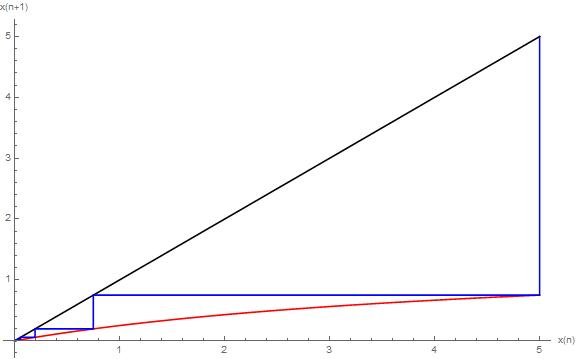
\includegraphics[width=4.5cm,height=4cm]{climbing1} &
        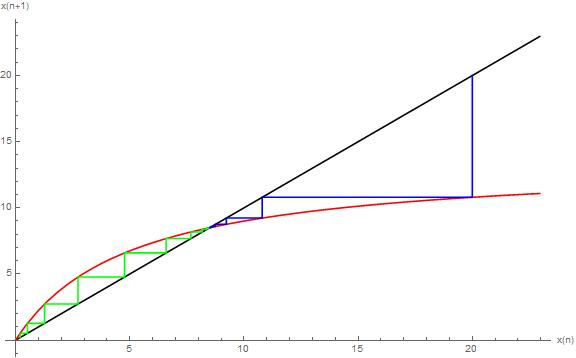
\includegraphics[width=6cm,height=4cm]{climbing2} \\
        {$0 < a \leq 1$} & {$a > 1$} \\
      \end{tabular}
    \end{figure}

  \end{center}

\end{frame}

\begin{frame}[t]{Ограниченост на популациите}

  \begin{block}{При Бевъртън-Холт мажориращи начални условия водят до мажориращи решения}
    Нека $x(n+1)=x(n)\frac{a}{b x(n) + 1}, a > 0, b > 0,x(0) \geq 0$. \\
    Параметризирайки по началното условие $x(0) = x_{0}$: \\
    $x(n+1,x_{0})= x(n,x_{0})\frac{a}{b x(n,x_{0}) + 1}, a > 0, b > 0,x(0, x_{0}) = x_{0} \geq 0$. \\
    Нека са дадени начални условия $\theta_{1}, \theta_{2}, \theta_{1} \geq \theta_{2}$. Тогава е в сила, че $\forall{n} \; x(n,\theta_{1}) \geq x(n,\theta_{2})$. Доказваме чрез индукция по $n$:
    \begin{itemize}
      \item $x(0, \theta_{1}) = \theta_{1} \geq \theta_{2} = x(0, \theta_{2})$
      \item $x(n+1, \theta_{1}) - x(n+1, \theta_{2}) =\frac{a x(n,\theta_{1})}{b x(n,\theta_{1}) + 1} - \frac{a x(n,\theta_{2})}{b x(n,\theta_{2}) + 1} = \frac{a (x(n,\theta_{1}) - x(n,\theta_{2}))}{b^{2} x(n,\theta_{1}) x(n,\theta_{2}) + b(x(n,\theta_{1}) + x(n,\theta_{2})) + 1} \geq 0$
    \end{itemize}

  \end{block}

\end{frame}

\begin{frame}[t]{Ограниченост на популациите}

  Достатъчно за четната подредица е да покажем, че $\forall{n} \; x_{1} \left(2n \right) + x_{2} \left(2n \right) < M$ за някое $M$, тъй като $x_{i} \left(2n \right) \geq 0 \implies x_{i} \left(2n \right) \leq x_{1} \left(2n \right) + x_{2} \left(2n \right) < M, \enspace i=1,2$. \\
  Допълнително, ограничеността на четната подредица влече ограничеността на нечетната:
  \[x_{i} \left(2n+1 \right) = x_{i} \left(2n \right) \frac{a_{i}}{1 + b_{i} x_{i} \left(2n \right)} \leq x_{i} \left(2n \right) a_{i} < a_{i} M = M_{i}', i=1, 2\]
  Тогава като дефинираме
  $M' = \max \{M_{1}',M_{2}',M\}$, то $\forall{n} \; x_{i} \left(n  \right) < M'$. \\

\end{frame}

\begin{comment}

\begin{frame}[t]{Ограниченост на популациите}

%Да допуснем, че $\exists{i \in \{1,2\}} \, \forall{M} \, \exists{n'} \, \forall{n \geq n'} \;  y_{i} \left(n \right) \geq M$. \\

%Случай 1: $\{y_{1}(n)\}_{n=0}^{\infty}, \{y_{2}(n)\}_{n=0}^{\infty}$ са неограничени. \\
%\quad Тогава, стига $y_{1}(n), y_{2}(n)$ да са достатъчно големи: $y_{1}(n+1)+y_{2}(n+1)=y_{1}(n) \frac{\alpha_{1} a_{1}}{(a_{1} \beta_{1} + b_{1}) y_{1}(n) + 1} + y_{2}(n) \frac{\alpha_{2} a_{2}}{(a_{2} \beta_{2} + b_{2}) y_{2}(n) + 1} \leq$ $\leq y_{1}(n)+y_{2}(n)$ \\
%Случай 2: Само $\{y_{i}(n)\}_{n=0}^{\infty}$ е неограничена.

Знаем, че: $y_{1}(n+1)+y_{2}(n+1)=y_{1}(n) \frac{\alpha_{1} a_{1}}{(a_{1} \beta_{1} + b_{1}) y_{1}(n) + 1} + y_{2}(n) \frac{\alpha_{2} a_{2}}{(a_{2} \beta_{2} + b_{2}) y_{2}(n) + 1}$ \\
Но сумата може да се замени от следната, оставайки същата: \\
$\xi_{1}(n+1)+\xi_{2}(n+1)=\xi_{1}(n) \frac{\alpha_{1} a_{1}}{(a_{1} \beta_{1} + b_{1}) \xi_{1}(n) + 1} + \xi_{2}(n) \frac{\alpha_{2} a_{2}}{(a_{2} \beta_{2} + b_{2}) \xi_{2}(n) + 1}$
Но може да дефинираме динамика за $\xi$:
\[\xi_{1}(n+1)=\xi_{1}(n) \frac{\alpha_{1} a_{1}}{(a_{1} \beta_{1} + b_{1}) \xi_{1}(n) + 1}\]
\[\xi_{2}(n+1)=\xi_{2}(n) \frac{\alpha_{2} a_{2}}{(a_{2} \beta_{2} + b_{2}) \xi_{2}(n) + 1}\]
Тук $\xi_{i}(0)=y_{i}(0),\enspace i=1,2$ \\
Сега свеждаме проблема до ограничеността на популация при стандартната динамика на Бевъртън-Холт.

\end{frame}

\end{comment}

\begin{frame}[t]{Ограниченост на популациите}

  Нека $A=\max \{\alpha_{1} a_{1},\alpha_{2} a{2}\}, B=\min \{a_{1} \beta_{1} + b_{1},a_{2} \beta_{2} + b_{2}\}$. Следва:
  $y_{i}(n+1) \leq y_{1}(n) \frac{A}{B y_{1}(n) + 1} + y_{2}(n) \frac{A}{B y_{2}(n) + 1}$. Тогава нека дефинираме динамиката за $\boldsymbol{\xi}$:
  \[\xi_{1}(n+1) = \xi_{1}(n) \frac{A}{B \xi_{1}(n) + 1} + \xi_{2}(n) \frac{A}{B \xi_{2}(n) + 1}, \enspace \xi_{1}(0)=y_{1}(0)\]
  \[\xi_{2}(n+1) = \xi_{1}(n) \frac{A}{B \xi_{1}(n) + 1} + \xi_{2}(n) \frac{A}{B \xi_{2}(n) + 1}, \enspace \xi_{2}(0)=y_{2}(0)\]
  Така $\forall{n} \; \xi_{i}(n) \geq y_{i}(n)$. Но $\forall{n} \; \xi_{1}(n+1)=\xi_{2}(n+1)$. Остава да проверим ограничеността на следната динамика:
  \[\hat{\xi}(n+1) = \hat{\xi}(n) \frac{2 A}{B \hat{\xi}(n) + 1}, \hat{\xi}(0)=\xi_{1}(0) \frac{A}{B \xi_{1}(0) + 1} + \xi_{2}(0) \frac{A}{B \xi_{2}(0) + 1}\]
  Но това е динамика на Бевъртън-Холт, която е ограничена по доказаното по-горе свойство.
  %Тя е ограничена, по показаното по-горе свойство, откъдето $\xi_{i}$ са ограничени, т.е. $y_{i}$ са ограничени и съответно $x_{i}$

\end{frame}


\begin{frame}[t]{Задача 4}
  Ако $\eta_{1} < \eta_{2} < 2$ не е изпълнено, възможно ли е популацията да оцелее? Изследвайте поведението на модела с помощта на числени симулации за
  избрани от вас стойности на параметрите.
\end{frame}


%\section{Числени симулации}

\captionsetup[figure]{labelformat=empty}

\begin{frame}[t]{Числени симулации - близък устойчив цикъл}

\begin{center}
\begin{figure}[htp]
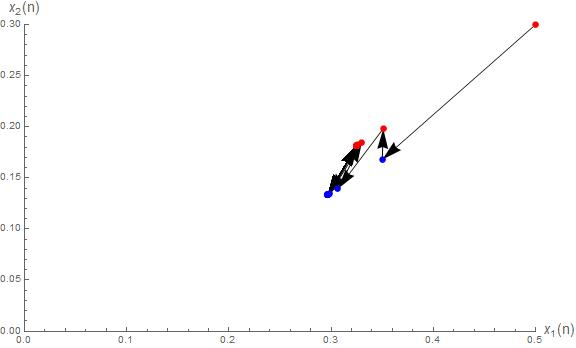
\includegraphics[width=8cm,height=6cm]{migrationSimulation1}
\caption{Развитие при $\eta_{1}=5.810, \eta_{2}=4.528$}
\end{figure}
\end{center}

\end{frame}

\begin{frame}[t]{Числени симулации - намаляване на препопулацията}

\begin{center}
\begin{figure}[htp]
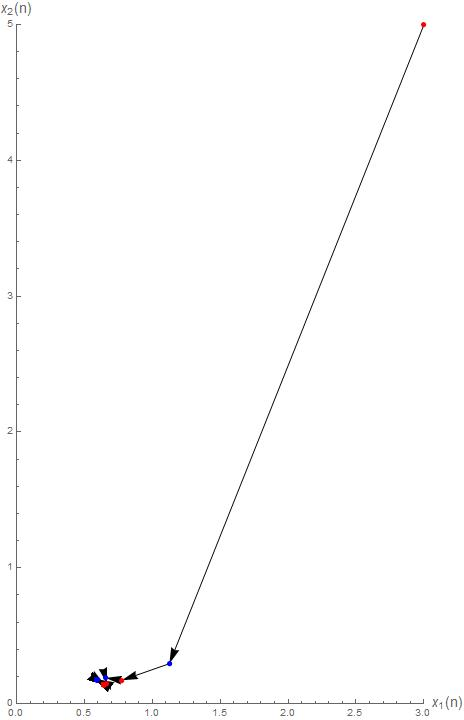
\includegraphics[width=5cm,height=7cm]
{migrationSimulation2}
\caption{Развитие при $\eta_{1}=4.200, \eta_{2}=-1.700$}
\end{figure}
\end{center}

\end{frame}

\begin{frame}[t]{Числени симулации - растеж до капацитета}

\begin{center}
\begin{figure}[htp]
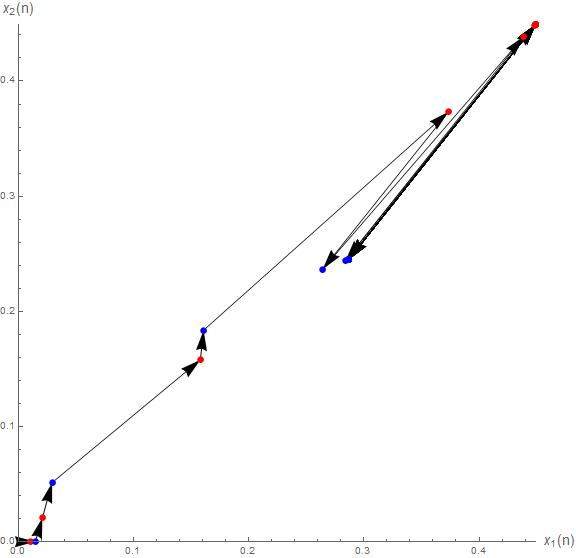
\includegraphics[width=6cm,height=6cm]
{migrationSimulation3}
\caption{Развитие при $\eta_{1}=12.75, \eta_{2}=1.000$}
\end{figure}
\end{center}

\end{frame}

\begin{frame}[t]{Числени симулации - $\eta_{1} < \eta_{2} < 2$}

\begin{center}
\begin{figure}[htp]
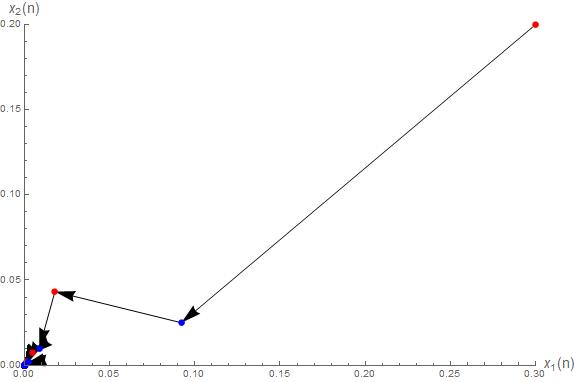
\includegraphics[width=9cm,height=7cm]
{migrationSimulation4}
\caption{Развитие при $\eta_{1}=0.154, \eta_{2}=0.971$}
\end{figure}
\end{center}

\end{frame}


\begin{frame}[t]{Заключение}

  Доказахме следните твърдения:
  \begin{enumerate}
    \item При адекватна параметризация, моделът е правдоподобен.
    \item Ако има индивиди в едното местообитание, то има и в другото.
    \item Популациите винаги са ограничени.
    \item Възможно е видът да изчезне и от двете местообитания.
    \item Изглежда, когато популациите не изчезват, гъстотите клонят към устойчив цикъл.
    \item Изглежда, че приближаването към устойчивите точки за всеки сезон е монотонно.

  \end{enumerate}

\end{frame}


{
\setbeamertemplate{headline}[default]
\begin{frame}

\begin{center}
\textbf{Благодаря за вниманието}
\end{center}

\end{frame}
}
\end{document}
